\section{9/10/2019}

\subsection{Bounding suprema via concentration}

The typical type of quantity we will focus on here is
\begin{align}
    \underbrace{\sup_{v \in V}}_{\text{bound by discretization}}
    \underbrace{\frac{1}{n} \sum_{i=1}^n \left(X_i(v) - \ex[X(v)] \right)}_{\text{bound for fixed $v$ via concentration}}\label{eq:typical-sup-via-concentration}
\end{align}
When $V$ is finite, a simple union bound can be applied.
To deal with infinitely large $\lvert V \rvert$, we will need to first discretize $V$ into
a finite set.

\subsection{Warmup: max of sub-Gaussian}

Suppose $\{X_i\}_{i=1}^n \simiid p$ where $p$ is mean zero and $\sigma$-sub-Gaussian.
How big is $\max_{i=1}^n X_i$?

\begin{lemma}\label{lem:concentration-max-sub-gaussian}
    With probability $\geq 1 - \delta$
    \begin{align}
        \max_{i=1}^n X_i \in O\left(\sigma \sqrt{\log n + \log \frac{1}{\delta}} \right)
    \end{align}
\end{lemma}

\begin{proof}
    By union bound, iid, and \nameref{eg:sub-gaussian-chernoff}
    \begin{align}
        \Pr\left[\max_{i=1}^n X_i \geq t \right]
        &\leq n \Pr[X_1 \geq t]
        \leq n \exp\left(-\frac{t^2}{2 \sigma^2}\right)
    \end{align}
    To ensure this failure event occurs with probability $\leq \delta$, we need
    \begin{align}
        n \exp\left(-\frac{t^2}{2 \sigma^2}\right) &\leq \delta \\
        \frac{t^2}{2 \sigma^2} &= \log n + \log \frac{1}{\delta} \\
        t &\leq \sigma \sqrt{2\left(\log n + \log \frac{1}{\delta} \right)}
    \end{align}
\end{proof}

If instead we were interested in $\max_{i=1}^n \lvert X_i \rvert$, then a union bound on the two
tail events $\{X_i \geq t\}$ and $\{-X_i \geq t\}$ (note $-X_i$ is still sub-Gaussian) gives
\begin{align}
    \Pr\left[\max_{i=1}^n \lvert X_i \rvert \geq t\right] &\leq 2 n \exp\left( -\frac{t^2}{2 \sigma^2} \right)
    \label{eq:tail-bound-abs-value-two-factor}\\
    \max_{i=1}^n \lvert X_i \rvert &\in O\left( \sigma \left(\sqrt{\log 2 + \log n + \log \frac{1}{\delta}}\right) \right)
\end{align}

In later the next section, we will see how we can ``reduce'' an infinitely large $V$
into an exponentially large $N$ after which
we will use the same technique to bound the event $\{ \max_{i \in N} X_i \geq t \}$.
To get concentration, we will need the exponential tail bound to dominate the now exponentially large $n = \lvert N \rvert$
arising from the union bound over $N$.

\subsection{Maximum eigenvalue of random matrix}

Suppose $\{X_i \in \RR^d \}_{i=1}^n \simiid p$ with $p$ zero mean and $\sigma$-sub-Gaussian.

Recall from \myref{def:orlicz-norm-multivar} and \myref{def:sub-gaussian-sub-exp-orlicz}
that $X \in \RR^d$ is $\sigma$-sub-Gaussian if all its one dimensional projections are, that is:
\begin{align}
    \|X\|_\psi + 1
    &= \sup_{v \in \cS^{d-1}} \|\braket{v,X}\|_\psi + 1
    = \sup_{v \in \cS^{d-1}} \ex \exp\left(\frac{\braket{v, X}^2}{\sigma^2} \right)
    \leq 2\label{eq:9-10-recap-multivar-sub-gaussian}
\end{align}

We are interested in the (random) empirical covariance matrix
\begin{align}
    M = \frac{1}{n} \sum_{i=1}^n X_i X_i^\top
\end{align}
Specifically, we would like to understand how big $\|M\| = \lambda_{\max}(M)$ is.

\begin{proposition}\label{prop:9-10-cov-operator-norm}
    With probability $\geq 1 - \delta$
    \begin{align}
        \|M\| = O\left(\sigma^2 \left( 1 + \frac{d}{n} + \frac{\log \frac{1}{\delta}}{n} \right) \right)
    \end{align}
\end{proposition}

\begin{remark}
    \Cref{prop:9-10-cov-operator-norm} shows that:
    \begin{itemize}
        \item As $n \to \infty$, $\|M\| = O(\sigma^2)$ and does not depend on $d$.
        \item The population covariance operator norm $\|\ex X_i X_i^\top\| = O\left( \frac{\sigma^2}{n} \log \frac{1}{\delta} \right)$ is attained if $d = \Theta(n)$ (i.e. if the dimension grows at the same rate as $n$)
    \end{itemize}
\end{remark}


To relate back to the two-step strategy outlined in \cref{eq:typical-sup-via-concentration}, note
\begin{align}
    \|M\| &= \sup_{v \in \cS^{d-1}} v^\top M v
    = \sup_{v \in \cS^{d-1}} \frac{1}{n} \sum_{i=1}^n \braket{X_i, v}^2
\end{align}
This quantity looks promising as it is the sum of independent sub-Gaussian RVs.

Since $\braket{X_i, v}$ is $\sigma$-sub-Gaussian, $\braket{X_i, v}^2$ is $\sigma^2$-sub-exponential (\cref{def:sub-gaussian-sub-exp-orlicz}, or equivalently \cref{eq:9-10-recap-multivar-sub-gaussian})
and for any fixed $v \in \cS^{n-1}$
\begin{align}
    \ex \exp\left(\frac{\braket{X_i, v}^2}{\sigma^2}\right) &\leq 2 \\
    \ex \exp\left(\frac{n}{\sigma^2} \frac{1}{n} \sum_{i=1}^n \braket{X_i, v}^2 \right)
    = \prod_{i=1}^n \ex \exp \left(\frac{\braket{X_i, v}^2}{\sigma^2}\right)
    &\leq 2^n
\end{align}
where we used \nameref{lem:mgf-sum-composition} for the equality in the second line.

By \cref{thm:chernoff}, for fixed $v \in \cS^{d-1}$
\begin{align}
    \Pr[v^\top M v \geq t] \leq 2^n \exp\left(\frac{-n t}{2 \sigma^2}\right) \label{eq:9-10-conc-sum}
\end{align}
So we have accomplished the first step (showing the individual terms inside the $\sup$ concentrate for fixed $v$).

For the second step, we will take a sufficiently small discretization of the unit ball $\{\|v\|\leq 1\}$:
\begin{lemma}\label{lem:9-10-unit-ball-packing}
    There exists a finite set $N \subset \RR^d$ with $\lvert N \rvert \leq 9^d$ and
    \begin{align}
        \sup_{v \in \cS^{d-1}} v^\top M v &\leq 2 \sup_{v \in N} v^\top M v
    \end{align}
\end{lemma}

Applying \cref{lem:9-10-unit-ball-packing}, a union bound, \cref{eq:9-10-conc-sum},
and bounding the failure probability by $\delta$
shows that
\begin{align}
    \Pr[ \|M\| \geq t ]
    &= \Pr\left[ \sup_{v \in \cS^{d-1}} v^\top M v \geq t \right]
    \leq 9^d 2^n \exp\left(\frac{-nt}{2 \sigma^2}\right) = \delta \\
    \frac{n t}{2 \sigma^2} &= d \log 9 + n \log 2 + \log \frac{1}{\delta} \\
    t &= O\left(\sigma^2 \left( \frac{d}{n} + 1 + \frac{\log 1/\delta}{n} \right)\right)
\end{align}

\begin{proof}[Proof of \cref{lem:9-10-unit-ball-packing}]
    Let $N$ be a maximal packing of $\Ball_1(0)$ in $\RR^d$
    such that $\|u - v\|_2 \geq \frac{1}{4}$ for all $u \neq v \in N$.

    As shown in \cref{fig:9-10-1}, if we place a $1/8$-radius ball at all the
    points in $N$ then (1) all the balls are disjoint and (2) the union of all the balls is
    contained in $\Ball_{9/8}(0)$ Therefore, by the (converse of the) pidgeonhole principle,
    $\lvert N \rvert \leq \frac{\Vol(\Ball_{9/8}(0))}{\Vol(\Ball_{1/8}(0))} = 9^d$.

    \begin{figure}[H]
        \centering
        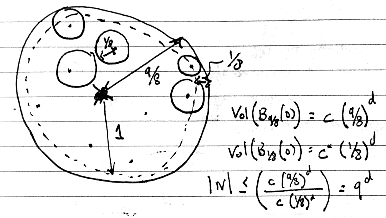
\includegraphics[width=0.6\textwidth]{figures/9-10-1.png}
        \caption{$1/8$-radius balls centered
            at all packing points are disjoint, the union of all these balls is contained in $B_{9/8}(0)$,
            so the cardinality $\lvert N \rvert \leq \left(\frac{9/8}{1/8}\right)^d = 9^d$.}
        \label{fig:9-10-1}
    \end{figure}

    Let $v \in \cS^{d-1}$ maximize $v^\top M v$
    and $u \in N$ such that $\|u - v\|_2 \leq \frac{1}{4}$.
    Such a $u$ must exist,
    otherwise $N \cup \{v\}$ is a larger $1/4$-packing which contradicts maximality of $N$.
    \begin{align}
        \|M\| - \lvert u^\top M u \rvert
        &= \lvert v^\top M v \rvert - \lvert u^\top M u \rvert \\
        &\leq \lvert v^\top M v - u^\top M u \rvert \\
        &= \lvert (u + v)^\top M (u - v) \rvert \\
        &\leq \underbrace{\|u + v\|_2}_{\leq 2} \|M\| \underbrace{\|u - v\|_2}_{\leq 1/4} \\
        &\leq \frac{1}{2} \|M\|
    \end{align}
    Hence $\|M\| \leq 2 u^\top M u \leq 2 \sup_{u \in N} u^\top M u$ as desired.
\end{proof}

\subsection{VC inequality and Symmetrization}

In this section, we will see how a family of events with certain geometric structure (which we will
quantify using VC-dimension) converges to its expectation at a rate dependent on the geometry.
In the process, we will encounter the technique of \emph{symmetrization}
(Prof. Steinhardt calls it ``bring your own randomness'') used to add additional randomness which
will be required to get concentration.

Let $\cH$ be a collection of functions $f : \cX \to \{0,1\}$ and $\{X_i \in \cX\}_{i=1}^n \simiid p$.
For $f \in \cH$, let
\begin{align}
    \nu(f) &= \ex_{x \sim p}[ f(x)] = \Pr_{x \sim p}[f(X) = 1] \\
    \nu_n(f) &= \frac{1}{n} \sum_{i=1}^n f(X_i) = \frac{1}{n} \#\{i : f(X_i) = 1\}
\end{align}
be the population and empirical averages respectively.

\textbf{Question}: How big is the discrepancy
\begin{align}
    D_n &= \sup_{f \in \cH} \lvert v_n(f) - v(f) \rvert
\end{align}

\textbf{Easy case}: $\lvert \cH \rvert < \infty$. Since $f(X_i)$ is bounded, apply \nameref{corr:hoeffding-inequality}
to the sum of independent bounded random variables to get:
\begin{align}
    D_n &= \max_{f \in \cH} \frac{1}{n} \sum_{i=1}^n (f(X_i) - \ex f(X)) \\
    \Pr\left[\frac{1}{n} \sum_{i=1}^n (f(X_i) - \ex f(X) \geq t \right] &\leq \exp(-2 n t^2)
\end{align}
A subsequent union bound over $\lvert \cH \rvert$ reveals
$t = O\left(\sqrt{\frac{1}{2n} \left( \log \lvert \cH \rvert + \log \frac{1}{\delta} \right)}\right)$

\textbf{More common case}: $\lvert \cH \rvert = \infty$.
In this situation, we will bound $D_n$ using the geometry of $\cH$.
To do so, we will quantify the geometry using the following definitions:

\begin{definition}[Shattering number / VC dimension]
    The \emph{shattering number} of $\cH$ is
    \begin{align}
        V_{\cH}(\{x_i\}_{i=1}^n) &= \text{\# distinct} \{(f(x_1), \ldots, f(x_n)) : f \in \cH\} \\
        V_{\cH}(n) &= \max_{\lvert S \rvert = n} V_{\cH}(S)
    \end{align}
    It measures the number of possible ways to assign $\{0,1\}$ labels to $x_i$ which can be perfectly
    fit by $f \in \cH$.

    The \emph{VC dimension}
    \begin{align}
        vc(\cH) &= \max\{ n : V_{\cH}(n) = 2^n\}\label{eq:vc-dim-def}
    \end{align}
    It measures the largest cardinality $n$ such that for any set of points $S$ with cardinality $\lvert S \rvert = n$
    and any $\{0,1\}$ labelling of those points, some $f \in \cH$ can perfectly fit it.
\end{definition}

The shattering number is useful because instead of taking $\sup_{f \in \cH}$ of a term
involving $f$ only through $\{f(X_i)\}_{i=1}^n$, we can instead take the supremum over
$\{f(X_i)\}_{i=1}^n$ directly and only deal with $V_{\cH}(n)$ terms.

\begin{example}[VC dimension of half spaces]\label{eg:half-spaces-vc}
    Let $\cX = \RR^d$, $\cH = \text{half spaces} = \{f(x) = \ind[\braket{v,x} \geq \tau] : v \in \RR^d, \tau \in \RR \}$.
    Then $vc(\cH) = d+1$.

    We will see a full proof later in \cref{prop:vc-dim-half-spaces}, but for
    now consider an example where $d=2$.
    We can always separate 3 points by drawing a line, so $vc(\cH) \geq 3$.
    However, with 4 points there can be crossings (see \cref{fig:9-10-vc-hs})
    which cannot be shattered.
    \begin{figure}[H]
        \centering
        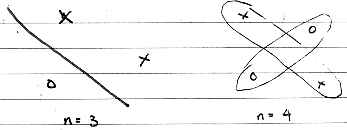
\includegraphics[width=0.6\textwidth]{figures/9-10-2.png}
        \label{fig:9-10-vc-hs}
        \caption{$n=3$ can always be shattered by a line, but the crossings possible when $n=4$ prevent this.}
    \end{figure}
\end{example}

Clearly by definition $V_\cH(n) = 2^n$ for all $n \leq vc(\cH)$.
When $n > vc(\cH)$, by \myref{eq:vc-dim-def} we have $V_\cH(n) < 2^n$.
The following lemma quantifies this and shows that the shattering number
is actually significantly smaller (growing polynomially in $n$ rather than exponentially):
\begin{lemma}[Sauer-Shelah]\label{lem:sauer-shelah}
    If $vc(\cH) = d$, then $V_{\cH}(n) \leq 2 n^d$.
\end{lemma}
While we will use this without proof, \nameref{lem:sauer-shelah} is the main reason why VC dimension
is useful for us: it allows us to convert the infinite supremum over $f \in \cH$ into a finite supremum over
$O(n^{\vc(\cH)})$ many terms of the form $\{f(X_i)\}_{i=1}^d$.

\begin{theorem}[VC inequality]\label{thm:vc-inequality}
    With probability $\geq 1 - \delta$
    \begin{align}
        D_n = O\left(\sqrt{\frac{vc(\cH) + \log \frac{1}{\delta}}{n}}\right)
    \end{align}
\end{theorem}

\begin{proof}
    We will show something weaker, namely:
    \begin{align}
        \ex D_n &\leq O\left( \frac{vc(\cH) \log n}{n} \right)
    \end{align}
    The $\log \frac{1}{\delta}$ tail bound follows from McDarmid's inequality,
    and removing the extra $\log n$ refines the argument we will give using a tool called chaining.

    \textbf{Incorrect proof path}: Notice that
    \begin{align}
        D_n &= \sup_{f \in \cH} \left\lvert
            \underbrace{\frac{1}{n} \sum_{i=1}^n (f(X_i) - \ex f(X))}_{\Pr[\cdot \geq t] \leq \exp(-2 n t^2)}
        \right\rvert
    \end{align}
    So \nameref{corr:hoeffding-inequality} can be used to control the term inside the supremum.
    Let $vc(\cH) = d$.
    By \cref{lem:sauer-shelah}, there are only $O(n^d)$ distinct $(f(X_1), \ldots, f(X_n))$
    so a union bound implies $t = O\left(\sqrt{\frac{d \log n + \log \frac{1}{\delta}}{2n}}\right)$

    This is incorrect because applying Sauer-Shelah requires us to condition on a specific realization of $\{X_i\}_{i=1}^n$
    (after which we know there are at most $V_{\cH}(n)$ distinct values of $(f(X_1), \ldots, f(X_n))$).
    After conditioning, there's no randomness left for applying \nameref{corr:hoeffding-inequality} to get concentration.

    \textbf{Solution}: Introduce additional randomness using \emph{symmetrization}.
    Introduce independent copies $X_i'$ and note
    \begin{align}
        \ex[D_n] &= \ex_{X_1, \ldots, X_n}\left[\sup_{f \in \cH} \left\lvert
            \frac{1}{n} \sum_{i=1}^n f(X_i) - \ex f(X)
        \right\rvert \right] \\
        &= \ex_{X_1, \ldots, X_n} \left[ \sup_{f \in \cH} \left\lvert \ex_{X_1', \ldots, X_n'} \left[
            \frac{1}{n} \sum_{i=1}^n (f(X_i) - f(X_i'))
        \right]\right\rvert\right]
    \end{align}
    $\lvert \cdot \rvert$ is convex, so by Jensen's inequality
    \begin{align}
        \ex[D_n]
        \leq \ex_{X} \left[ \sup_{f \in \cH} \ex_{X'} \left[\left\lvert
            \frac{1}{n} \sum_{i=1}^n (f(X_i) - f(X_i'))
        \right\rvert \right]\right]
    \end{align}
    Also, $\sup_y \ex f(X,y) \leq \ex \sup_y f(X,y)$ for any function $f$
    (since $\ex f(X,y) \leq \ex \sup_y f(X,y)$ then take supremum on left-hand side, or see Fatou-Lebesgue theorem)
    hence we can move $\ex_{X'}$ out of $\sup_{f \in \cH}$ to get
    \begin{align}
        \ex[D_n]
        &\leq \ex_{X, X'}\left[
        \sup_{f \in \cH} \left\lvert \frac{1}{n} \sum_{i=1}^n ( f(X_i) - f(X_i') )
        \right\rvert\right]
    \end{align}
    Here is where the randomness from symmetrization is added:
    since $f(X_i) - f(X_i') \overset{d}{=} \eps_i(f(X_i) - f(X_i'))$ for $\eps_i \sim \text{Rad}$
    \begin{align}
        \ex[D_n]
        &\leq \ex_{X, X', \eps}\left[
        \sup_{f \in \cH} \left\lvert \frac{1}{n} \sum_{i=1}^n \eps_i ( f(X_i) - f(X_i') )
        \right\rvert\right] \label{eq:9-10-symmetrized-need-concentration}
    \end{align}
    Condition on $X, X'$ and let $f(X_i) = a \in V_{\cH}(\{x_1, \ldots, x_n\})$
    and $f(X_i') = b \in V_\cH(\{x_1', \ldots, x_n'\})$. Then
    \begin{align}
        \sup_{f \in \cH}
            \left\lvert \frac{1}{n} \sum_{i=1}^n \eps_i(f(X_i) - f(X_i')) \right\rvert
        &= \sup_{a, b}
            \underbrace{
                \left\lvert \frac{1}{n} \sum_{i=1}^n \eps_i (a_i - b_i)\right\rvert
            }_{\Pr[\lvert \cdot \rvert \geq t] \leq 2 \exp(\frac{-n t^2}{2})}
    \end{align}
    Now we can apply \nameref{corr:hoeffding-inequality} (picking up an extra factor of $2$ because
    of the absolute value, see \cref{eq:tail-bound-abs-value-two-factor}) to the independent,
    zero-mean (since $\ex \eps_i = 0$),
    bounded (since $a_i$, $b_i$, and $\eps_i$ are all bounded)
    random (since $\eps_i$ is still random) variables
    and union bound over the $O(n^{2d})$ (by \nameref{lem:sauer-shelah}, squared since there is both $f(X)$ and $f(X')$) distinct $f(X)$ and $f(X')$
    \begin{align}
        \Pr\left[ \sup_{f \in \cH}
            \left\lvert \frac{1}{n} \sum_{i=1}^n \eps_i(f(X_i) - f(X_i')) \right\rvert \geq t
        \middle| X, X' \right]
        &\leq (2 n^{2d}) 2 \exp\left(\frac{-n t^2}{2} \right) \\
    \end{align}
    This tail probability is small if $t \gg \sqrt{\frac{d \log n}{n}}$, so \todo{why?? Try $\ex X = \int P(X \geq t) dt$ for $X \geq 0$}
    the expectation over $\eps$ in \cref{eq:9-10-symmetrized-need-concentration} is of the same order
    and we have
    \begin{align}
        \ex[D_n]
        &\leq \ex_{X, X'}\left[
            \ex_{\eps}\left[
                \sup_{f \in \cH} \left\lvert \frac{1}{n} \sum_{i=1}^n \eps_i ( f(X_i) - f(X_i') )
                \middle| X, X'\right]
        \right\rvert\right]
        = O\left(
            \sqrt{\frac{d \log n}{n}}
        \right)
    \end{align}
\end{proof}

Discretization to a representative set (``fingerprinting'') is how previous sections worked.
The complication here is that to apply \cref{lem:sauer-shelah} we had to condition on $X_i$ and
remove the randomness. The secret sauce was to add randomness back using the $\eps_i$ in
symmetrization.
